\subsubsection{Dimensionality Reduction Analysis}
\label{subsubsec:discussion-reduction}

This section examines the impact of three reduction techniques—GGCN, ENNTH, and Drop3—on the performance, training time, testing time, and storage requirements of both the KNN and SVM algorithms.



% Add more content here as needed

% KNN Reduction hepatitis vs. KNN Reduction mushroom
% Time
% Space
\begin{figure}
    \centering
    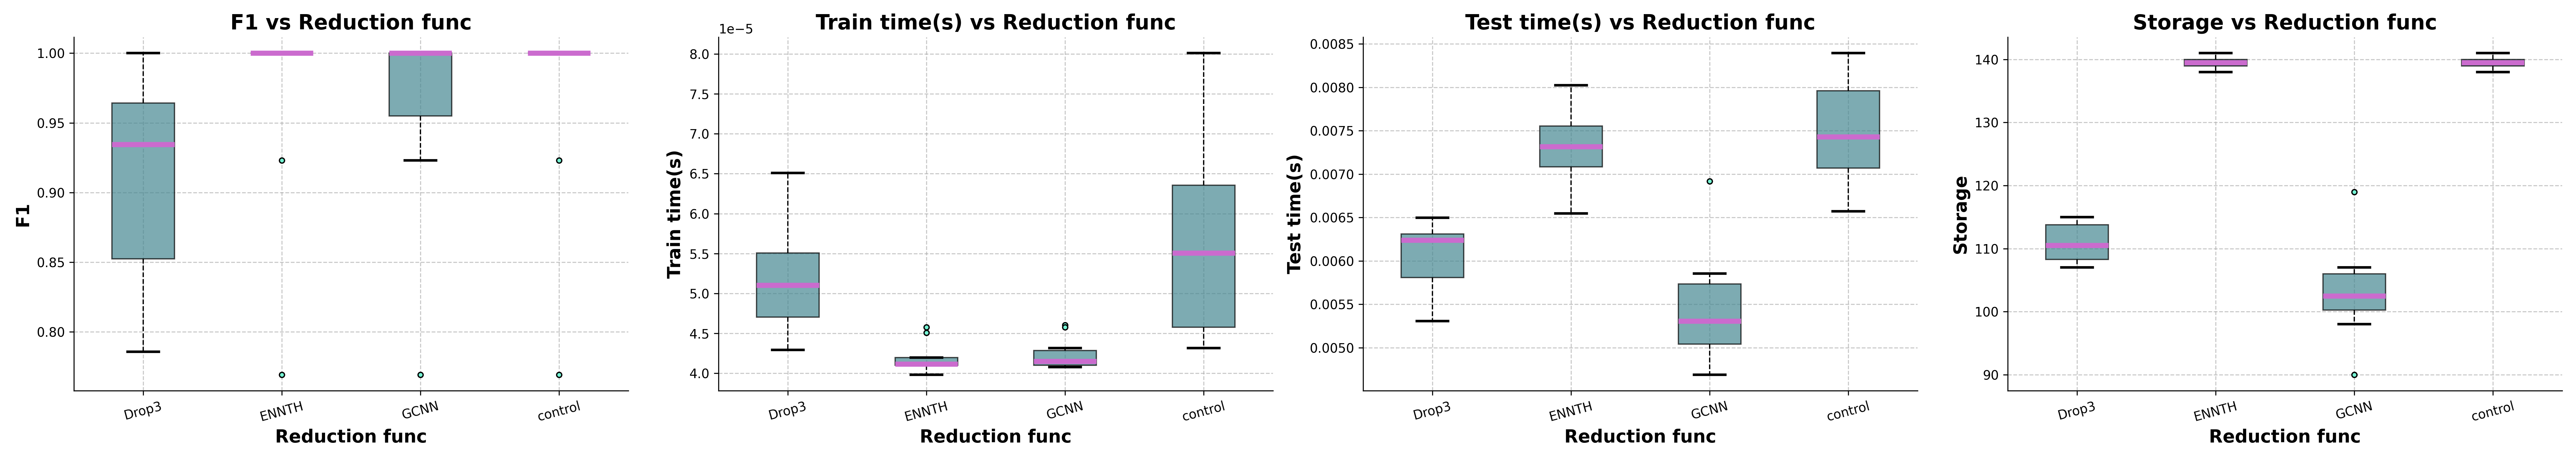
\includegraphics[width=0.45\textwidth]{figures/work2/reports/figures/KNN_reduction_effects_hepatitis.png}
    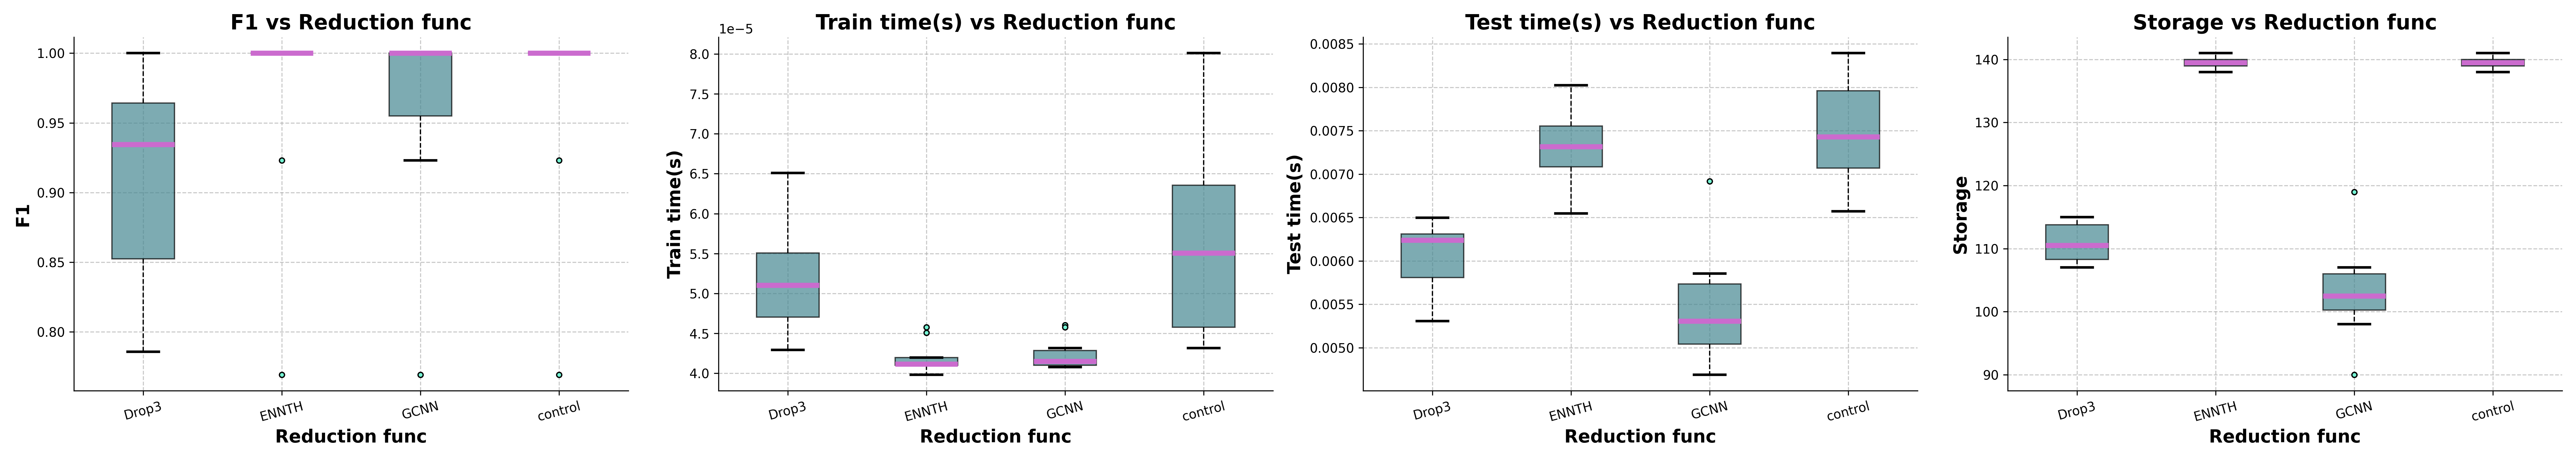
\includegraphics[width=0.45\textwidth]{figures/work2/reports/figures/KNN_reduction_effects_hepatitis.png}
    \caption{Class distributions}
    \label{fig:class-distributions}
\end{figure}

% SVM Reduction hepatitis vs. KNN Reduction mushroom
% Time
% Space
\begin{figure}
    \centering
    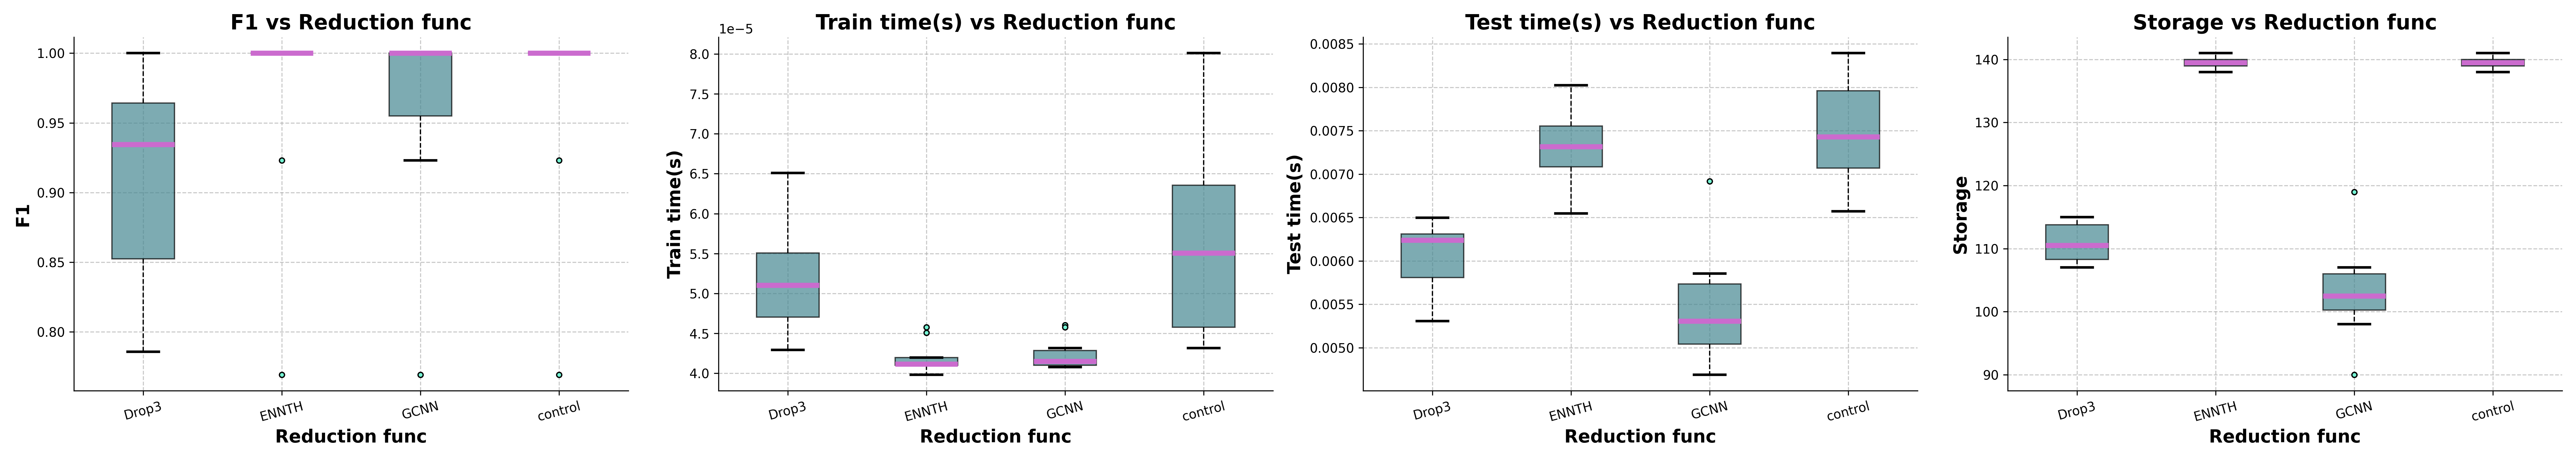
\includegraphics[width=0.45\textwidth]{figures/work2/reports/figures/KNN_reduction_effects_hepatitis.png}
    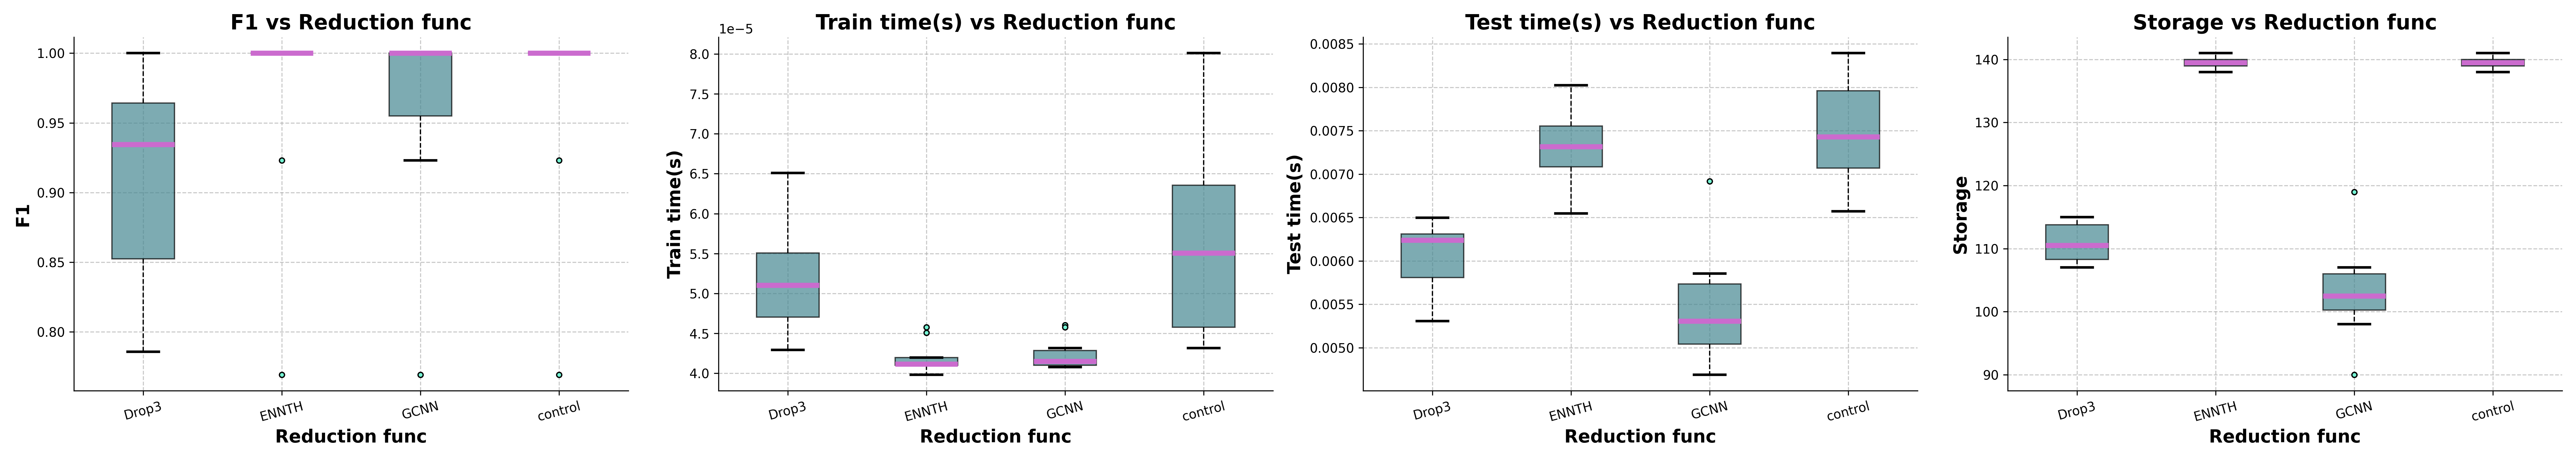
\includegraphics[width=0.45\textwidth]{figures/work2/reports/figures/KNN_reduction_effects_hepatitis.png}
    \caption{Class distributions}
    \label{fig:class-distributions}
\end{figure}


